%! TeX program = lualatex
\documentclass[a4paper]{article} 

% packages
\usepackage{microtype}      % Slightly tweak font spacing for aesthetics
\usepackage[english]{babel} % Language hyphenation and typographical rules
\usepackage{changepage}     % adjust margins on the fly
\usepackage{booktabs}  % For better-looking tables
\usepackage{pgfplotstable}  % For reading and displaying CSV/TSV files
\usepackage{appendix}

\usepackage[final, colorlinks = true, urlcolor = black, linkcolor = black, citecolor = black]{hyperref} 
\usepackage{fontspec}
% \setmainfont{EB Garamond}
% \setmonofont[Scale=MatchLowercase]{Deja Vu Sans Mono}

\setmainfont{EB Garamond}[
    Ligatures=TeX,
    Numbers=OldStyle
]

% Fallback font (for missing characters)
\setmainfont{EB Garamond}[
    % Ligatures=TeX,
    % Numbers=OldStyle
]

\newfontfamily{\emojifont}{Noto Color Emoji}[Renderer=Harfbuzz]

% Monospace font configuration
\setmonofont[Scale=MatchLowercase]{DejaVu Sans Mono}

\usepackage[backend=biber, style=numeric, date=iso, urldate=iso]{biblatex}
\addbibresource{references.bib}
\DeclareFieldFormat{urldate}{Accessed on: #1}

\usepackage{minted}
\usemintedstyle{algol_nu}
\usepackage{xcolor}

\usepackage{pgfplots}
\pgfplotsset{width=\textwidth,compat=1.9}

\usepackage{caption}
\newenvironment{code}{\captionsetup{type=listing}}{}
\captionsetup[listing]{skip=0pt}
\setlength{\abovecaptionskip}{5pt}
\setlength{\belowcaptionskip}{5pt}

\usepackage[yyyymmdd]{datetime}
\renewcommand{\dateseparator}{--}

\usepackage{titlesec}
% \titleformat{\section}{\LARGE\bfseries}{}{}{}[\titlerule]
% \titleformat{\subsection}{\Large\bfseries}{}{0em}{}
% \titlespacing{\subsection}{0em}{-0.7em}{0em}
%
% \titleformat{\subsubsection}{\large\bfseries}{}{0em}{$\bullet$ }
% \titlespacing{\subsubsection}{1em}{-0.7em}{0em}

% margins
\addtolength{\hoffset}{-2.25cm}
\addtolength{\textwidth}{4.5cm}
\addtolength{\voffset}{-3.25cm}
\addtolength{\textheight}{5cm}
\setlength{\parskip}{0pt}
\setlength{\parindent}{0in}
% \setcounter{secnumdepth}{0}

\begin{document}
\hrule \medskip
\begin{minipage}{0.295\textwidth} 
    \raggedright
    \footnotesize 
    \begin{tabular}{@{}l l}
        Name: & Andrew Hayes \\
        Student ID: & 21321503 \\
        E-mail: & \href{mailto://a.hayes18@universityofgalway.ie}{\texttt{a.hayes18@universityofgalway.ie}} \\
    \end{tabular}
\end{minipage}
\begin{minipage}{0.4\textwidth} 
    \centering 
    \vspace{0.4em}
    \LARGE
    \textsc{ct414} \\ 
\end{minipage}
\begin{minipage}{0.295\textwidth} 
    \raggedleft
    \today
\end{minipage}
\medskip\hrule 
\begin{center}
    \normalsize
    Assignment 2: MapReduce
\end{center}
\hrule
\medskip

\section{Set-Up}
To obtain large text files to test the program with, I downloaded the first 10 long books I could think of from \url{archive.org} in \verb|txt| file form.
These were:
\begin{enumerate}
    \item   The Bible;
    \item   \textit{War \& Peace} by Leo Tolstoy;
    \item   Plutarch's \textit{Lives};
    \item   Herodotus' \textit{Histories};
    \item   \textit{City of God} by Augustine of Hippo;
    \item   \textit{Faust} by Goethe;
    \item   \textit{Wealth of Nations} by Adam Smith;
    \item   \textit{Capital} by Karl Marx;
    \item   The complete works of William Shakespeare;
    \item   \textit{Structure \& Interpretation of Computer Programs} by Harold Abelson \& Gerald Jay Sussman.
\end{enumerate}

\section{Baseline Results}
I modified the code to measure \& output the time taken by each approach, in milliseconds.
I also added timing for the different phases of the two MapReduce implementations, timing the map time, group time, and reduce time separately.

\begin{figure}[H]
    \centering
    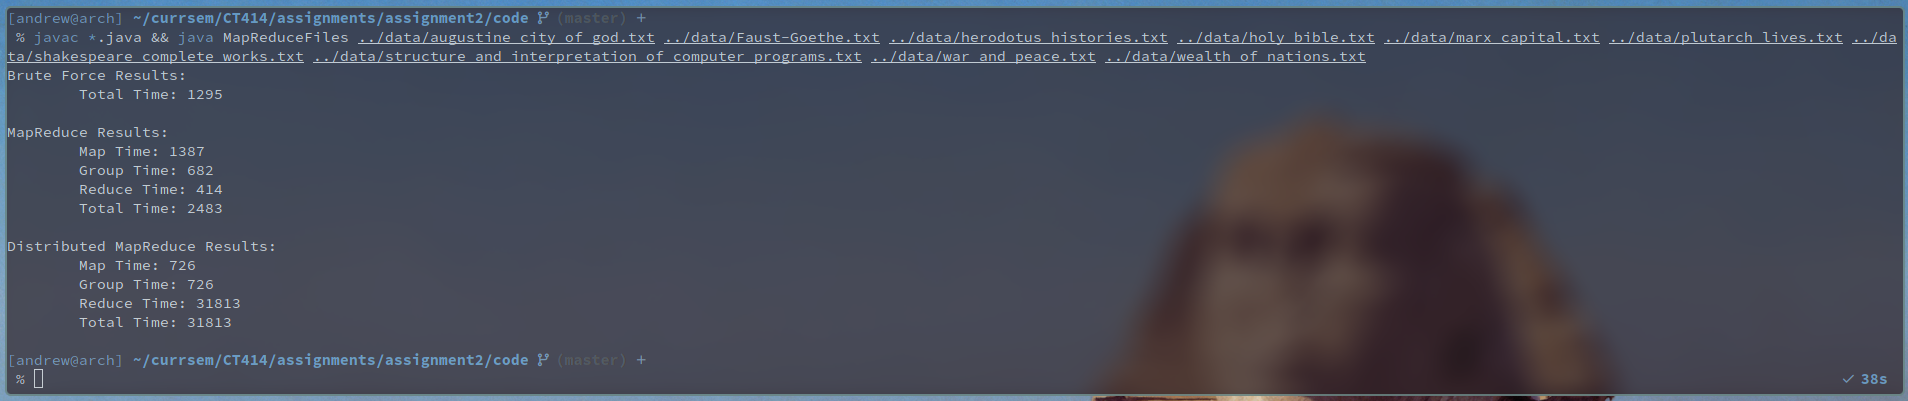
\includegraphics[width=\textwidth]{./images/baseline.png}
    \caption{Baseline results for my list of files (in milliseconds)}
\end{figure}

As can be seen from the above terminal screenshot, the brute force approach performed best with no modifications, followed by the non-distributed MapReduce, followed by the distributed MapReduce;
this is to be expected, as the brute force approach is the simplest \& requires the fewest iterations over the data and no complex data structures.
The non-distributed MapReduce requires more intermediate data structure and more iterations over the data.
Finally, the non-optimised version of the distributed MapReduce is the slowest because it spawns a thread for each word in the dataset, causing massive stress on the CPU and memory.
\\\\
I also updated the code to use \mintinline{java}{ArrayList}s rather than \mintinline{java}{LinkedList}s to reduce memory overhead and have faster traversal.

\begin{figure}[H]
    \centering
    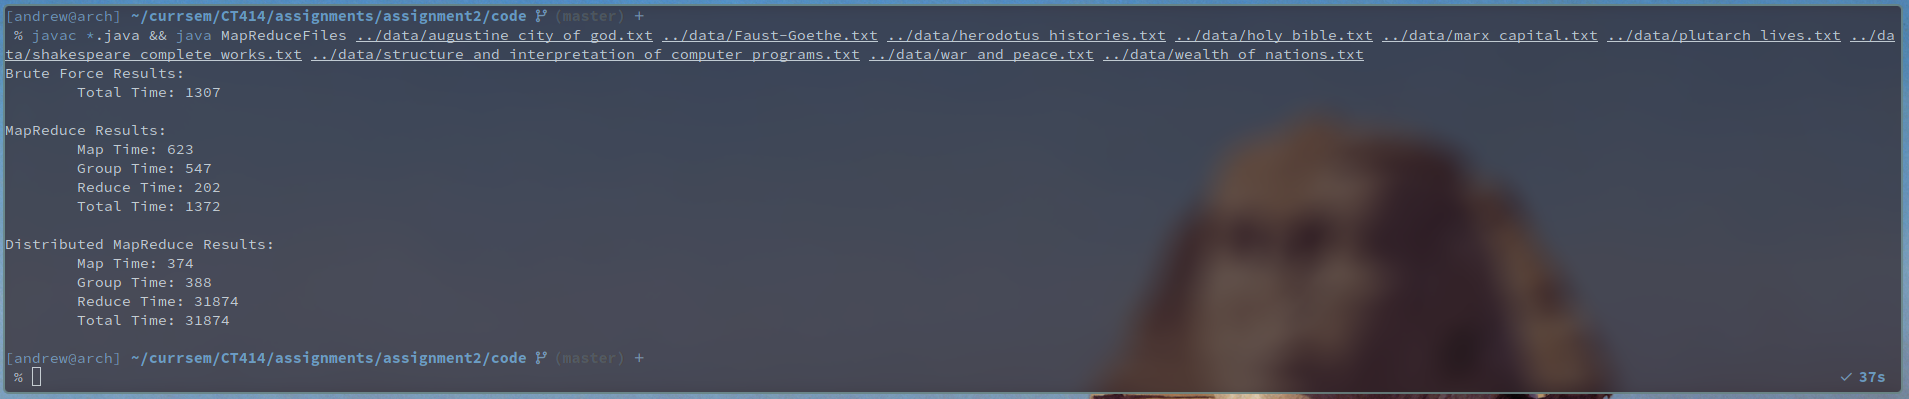
\includegraphics[width=\textwidth]{./images/arraylist.png}
    \caption{Baseline results with \mintinline{java}{ArrayList} update (in milliseconds)}
\end{figure}

As can be seen from the above terminal screenshot, this has no affect on the brute force results (besides slight variance due to background processes running on my laptop) as this approach did not use \mintinline{java}{LinkedList}s anyway.
The non-distributed MapReduce approach was significantly faster due to the faster iteration and lower memory overhead.
The distributed MapReduce saw significant improvements in the map \& group phases, but these were dwarfed by the still greatly inefficient reduce phase.

\section{Testing the Updated Code}
After implementing the requested changes in steps 2--6 of the assignment specification, I then implemented a grid-search function which tested a range of values for the number of lines of text per map thread and the number of words per reduce thread.
The results of this grid-search were exported to a CSV file for analysis.
I then wrote a Python script to visualise the parameter combinations using heatmaps.

\begin{figure}[H]
    \centering
    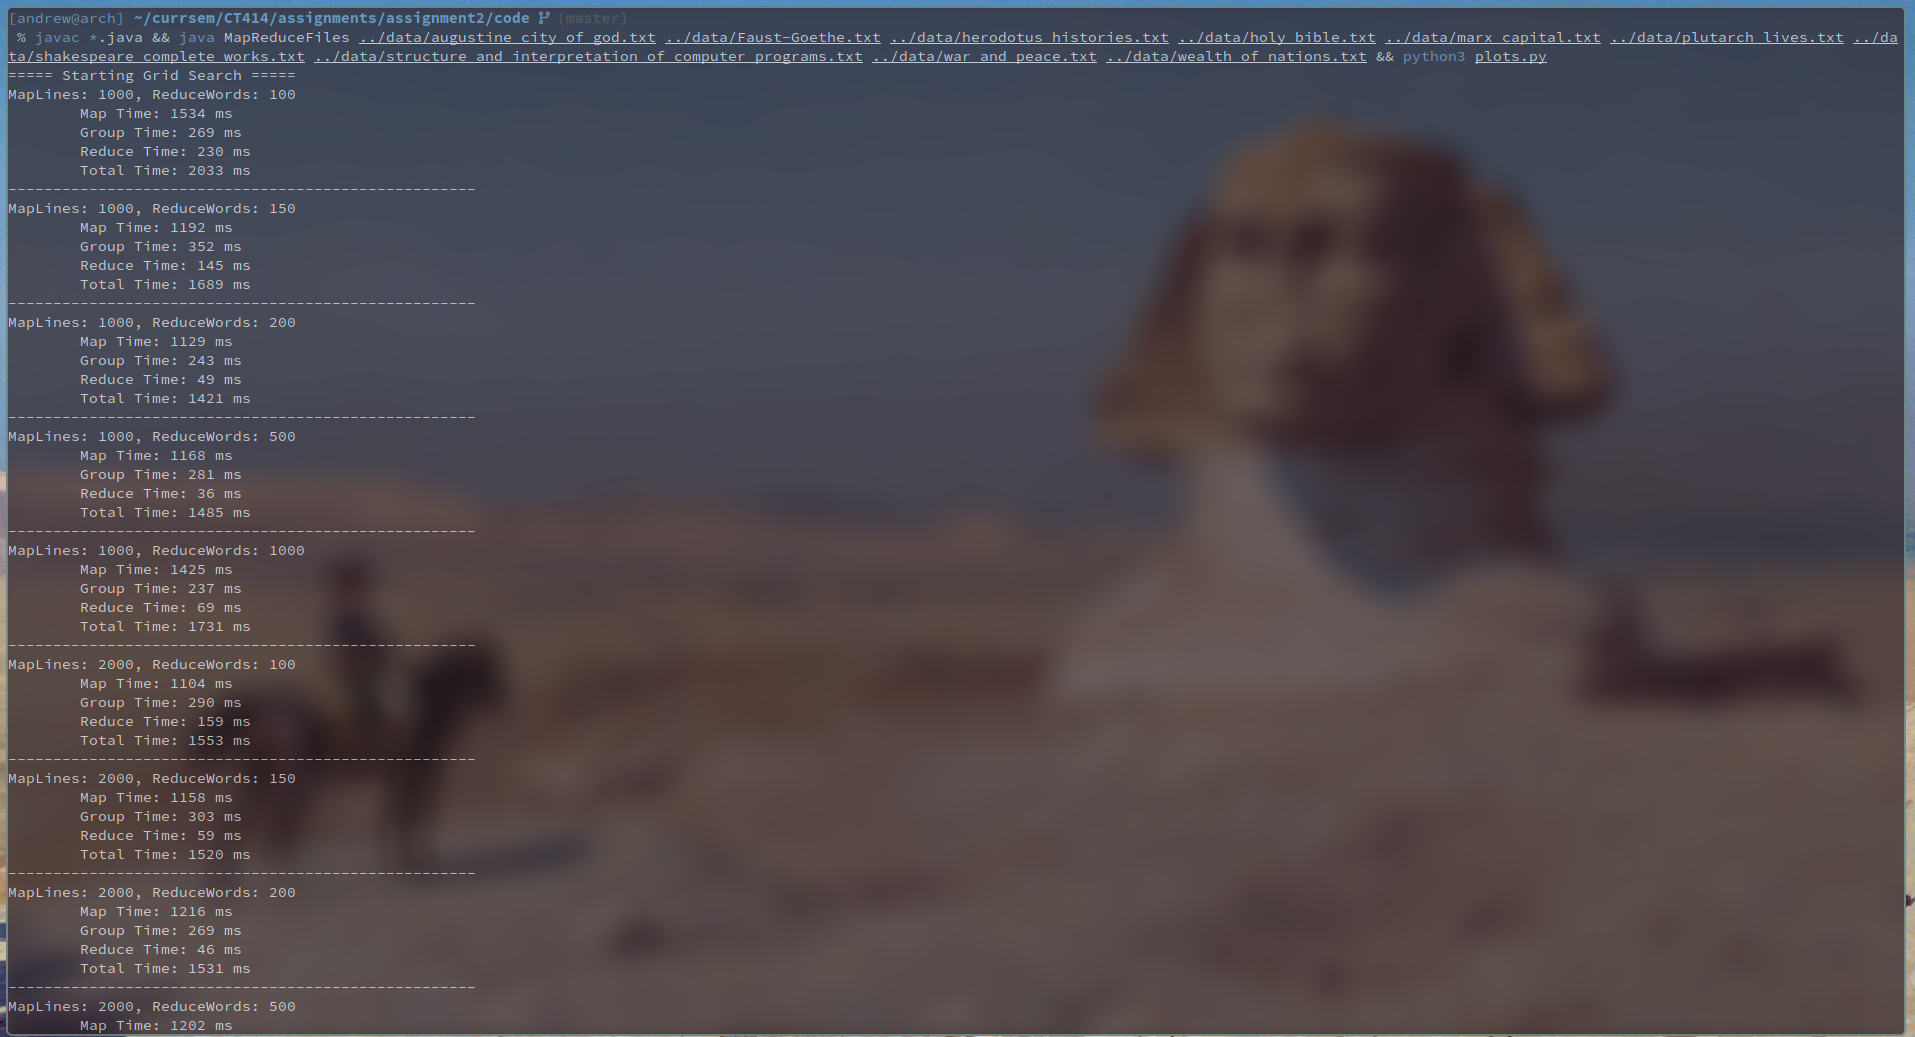
\includegraphics[width=\textwidth]{./images/gridsearch.png}
    \caption{Running the grid-search and plotting the results}
\end{figure}

\begin{table}[H]
\centering
\pgfplotstabletypeset[
    col sep=comma,
    string type,
    header=true,
    columns/MapLines/.style={column name=Map Lines},
    columns/ReduceWords/.style={column name=Reduce Words},
    columns/MapTime/.style={column name=Map Time (ms)},
    columns/GroupTime/.style={column name=Group Time (ms)},
    columns/ReduceTime/.style={column name=Reduce Time (ms)},
    columns/TotalTime/.style={column name=Total Time (ms)},
    every head row/.style={before row=\toprule, after row=\midrule},
    every last row/.style={after row=\bottomrule}
]{../code/performance_results.csv}
\caption{Results written to \texttt{performance\_results.csv}}
\end{table}


\begin{figure}[H]
    \centering
    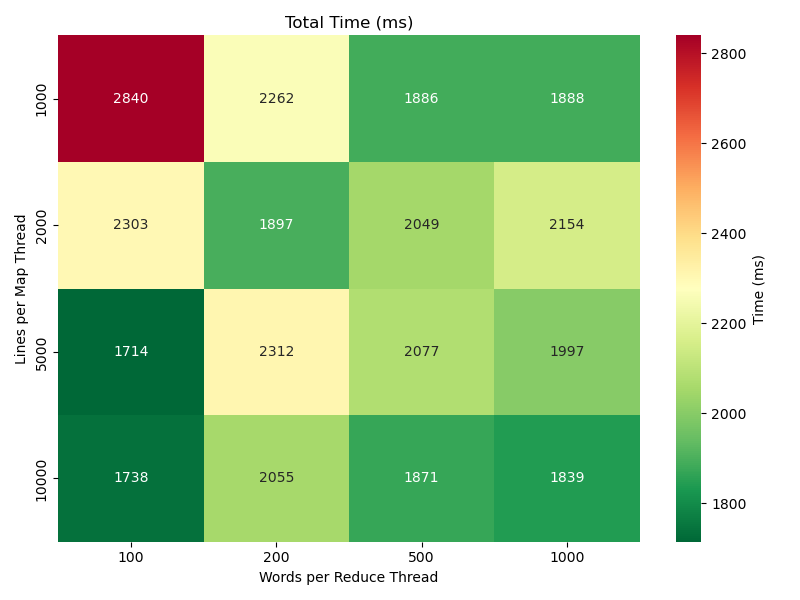
\includegraphics[width=0.8\textwidth]{./images/total_time_heatmap.png}
    \caption{Heatmap of total time taken by each parameter combination}
\end{figure}

\begin{figure}[H]
    \centering
    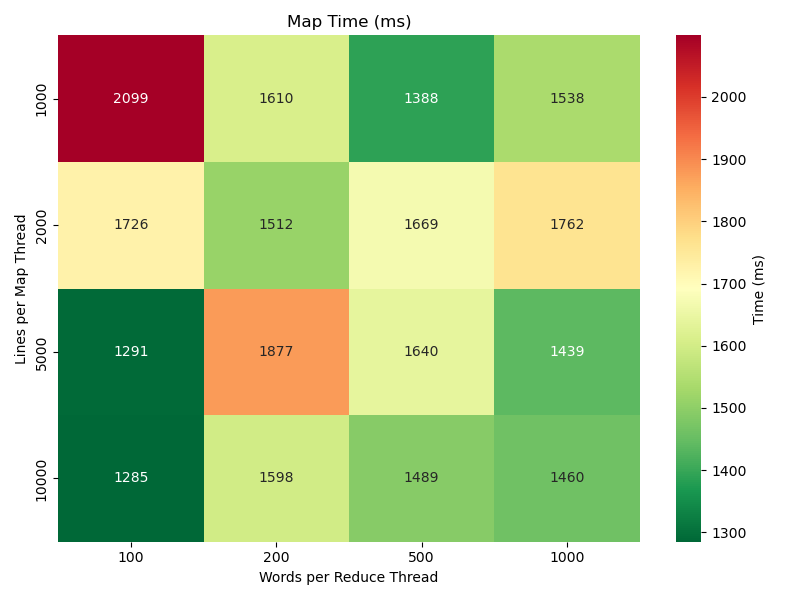
\includegraphics[width=0.8\textwidth]{./images/map_time_heatmap.png}
    \caption{Heatmap of time taken during the map phase by each parameter combination}
\end{figure}

\begin{figure}[H]
    \centering
    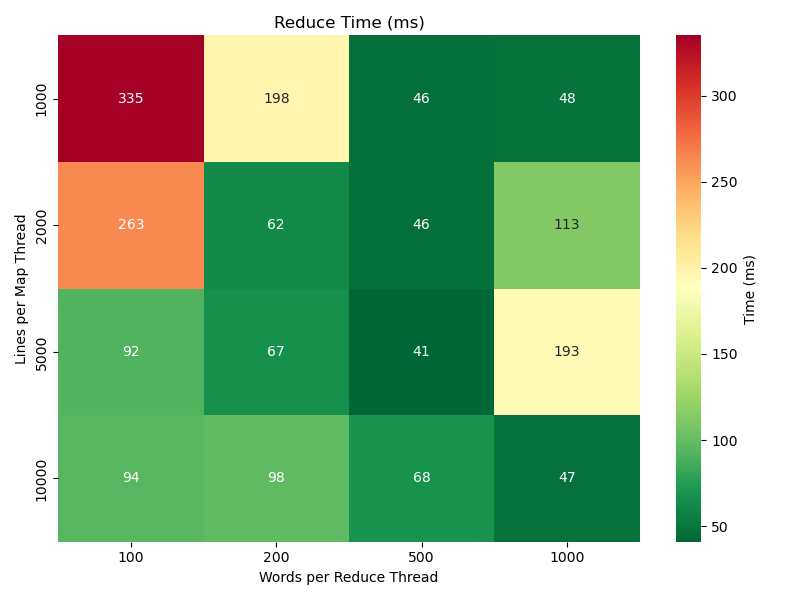
\includegraphics[width=0.8\textwidth]{./images/reduce_time_heatmap.png}
    \caption{Heatmap of time taken during the reduce phase by each parameter combination}
\end{figure}

\section{Appendix: Source Code}
\begin{code}
    \inputminted[linenos, breaklines, frame=single]{java}{../code/MapReduceFiles.java}
    \caption{\texttt{MapReduceFiles.java}}
\end{code}

\begin{code}
    \inputminted[linenos, breaklines, frame=single]{python}{../code/plots.py}
    \caption{\texttt{plots.py}}
\end{code}




\end{document}
